\section {Применение имитационного моделирования в теории массового обслуживания}
Имитационное моделирование \cite{задорожный2011методы} является мощным инструментом для экспериментального изучения систем массового обслуживания. Его актуальность как метода исследования обусловлена следующими факторами:
\begin{enumerate}
	\item принцип, лежащий в основе моделирования, довольно прост для понимания, что делает этот инструмент доступным для широкого круга исследователей, в том числе для тех, кто не имеет глубоких познаний в теории случайных процессов;
	\item при использовании имитационного моделирования в связке со сложными средствами визуализации можно детально наблюдать процесс работы системы в различных ее аспектах, что дает данные, которые невозможно получить при помощи исключительно численного подхода к анализу, более сфокусированного на различных показателях функционирования системы; 
	\item численные методы в большинстве случаев опираются на решение специально составленных систем уравнений (система уравнений Колмогорова). В свою очередь, имитационное моделирование предлагает методологию, которая помогает рассчитать те же показатели без изменения основного подхода \cite{glynn1988simulation};
	\item имитационное моделирование зачастую является способом подтвердить аналитические результаты, при исследовании системы массового обслуживания методом асимптотического анализа и определить их область применимости. Поскольку в качестве аналитического решения, как правило, выступает аппроксимация некой функции, то для установки ее качества требуется применение численных методов исследования, среди которых имитационное моделирование предоставляет широкий набор возможностей.
\end{enumerate}

Система массового обслуживания описывает при помощи специального математического аппарата \cite{nazarov2010theory} порядок обработки заявок --- абстрактных объектов, которые в реальном мире могут выступать в качестве телефонных звонков, сетевых запросов или клиентов, требующих обслуживания. Для описании работы системы используется ряд основных элементов, которые проводят операции над заявками:
\begin{enumerate}
	\item входящий поток --- является случайным потоком событий (заявок), возникающих в системе и требующих обработки;
	\item обслуживающий прибор --- второй важный элемент системы массового обслуживания, представляющий собой случайных процесс обработки заявок. В системе может быть несколько приборов, при том их блок может также иметь различную топологию: они могут обслуживать заявки последовательно, либо параллельно. Также на конфигурацию системы влияет и выбор самого количества обслуживающих приборов;
	\item Для описания класса систем массового обслуживания, в которых заявок может не суметь получить доступ к прибору, используется источник повторных вызовов, иначе орбита, которая агрегирует заявки, которые не смогли захватить прибор и через некоторое случайное время попытаются повторить попытку захвата
	\item Для регулирования поступления заявок на прибор используется очередь, иначе буфер, которая накапливает входящие заявки прежде чем они попадут на прибор.
\end{enumerate} 

Все перечисленные элементы являются случайными процессами и могут иметь различные характеристики и распределение случайных величин. Задачей теории массового обслуживания является выбор наиболее эффективной структуры системы для ее наилучшей производительности. Данная задача решается путем нахождения и анализа характеристик ее функционирования. Среди аналитических методов решения этой задачи можно выделить метод асимптотического анализа \cite{назаров1991асимптотический} и метод диффузионного анализа \cite{назаров2021исследование}. Имитационное моделирование, в свою очередь, является как методом апробации полученных аналитических результатов при помощи численных экспериментов, так и подходом к исследованию систем массового обслуживания, заключающимся в имитации работы исследуемой модели системы массового обслуживания посредством компьютерных вычислений. 

Как упомянуто выше, ключевое преимущество имитационного моделирования --- прямолинейная реализация алгоритма, что экономит время и снижает трудоемкость исследования. Из относительно простой реализации алгоритмов вытекает и легкое конфигурирование и изменение структуры системы с возможностью быстрого получения результатов в последствии.

При моделировании систем массового обслуживания используется дискретно-событийный подход. Он заключается в генерации случайных величин, имеющих требуемое распределение, которые являются моментами наступления событий в системе. События могут быть различного рода: окончание обслуживания заявки, перемещение заявки на прибор, поломка прибора и т. д. В момент наступления события состояние системы меняется, что и отслеживается в процессе моделирования.

Рассмотрим подход подробнее на примере следующей системы:

на вход системы поступает пуассоновский поток заявок. Заявка занимает прибор в случае, если он свободен, тот, в свою очередь, начинает ее обслуживание в течение экспоненциально распределенного времени с параметром $\mu$. В ситуации, когда прибор уже занят обслуживанием, входящая заявка, после неудавшейся попытки захватить прибор, мгновенно уходит на орбиту и осуществляет там случайную задержу в течение экспоненциально распределенного времени с параметром $\sigma$.

\begin{figure}[H]
	\centering
	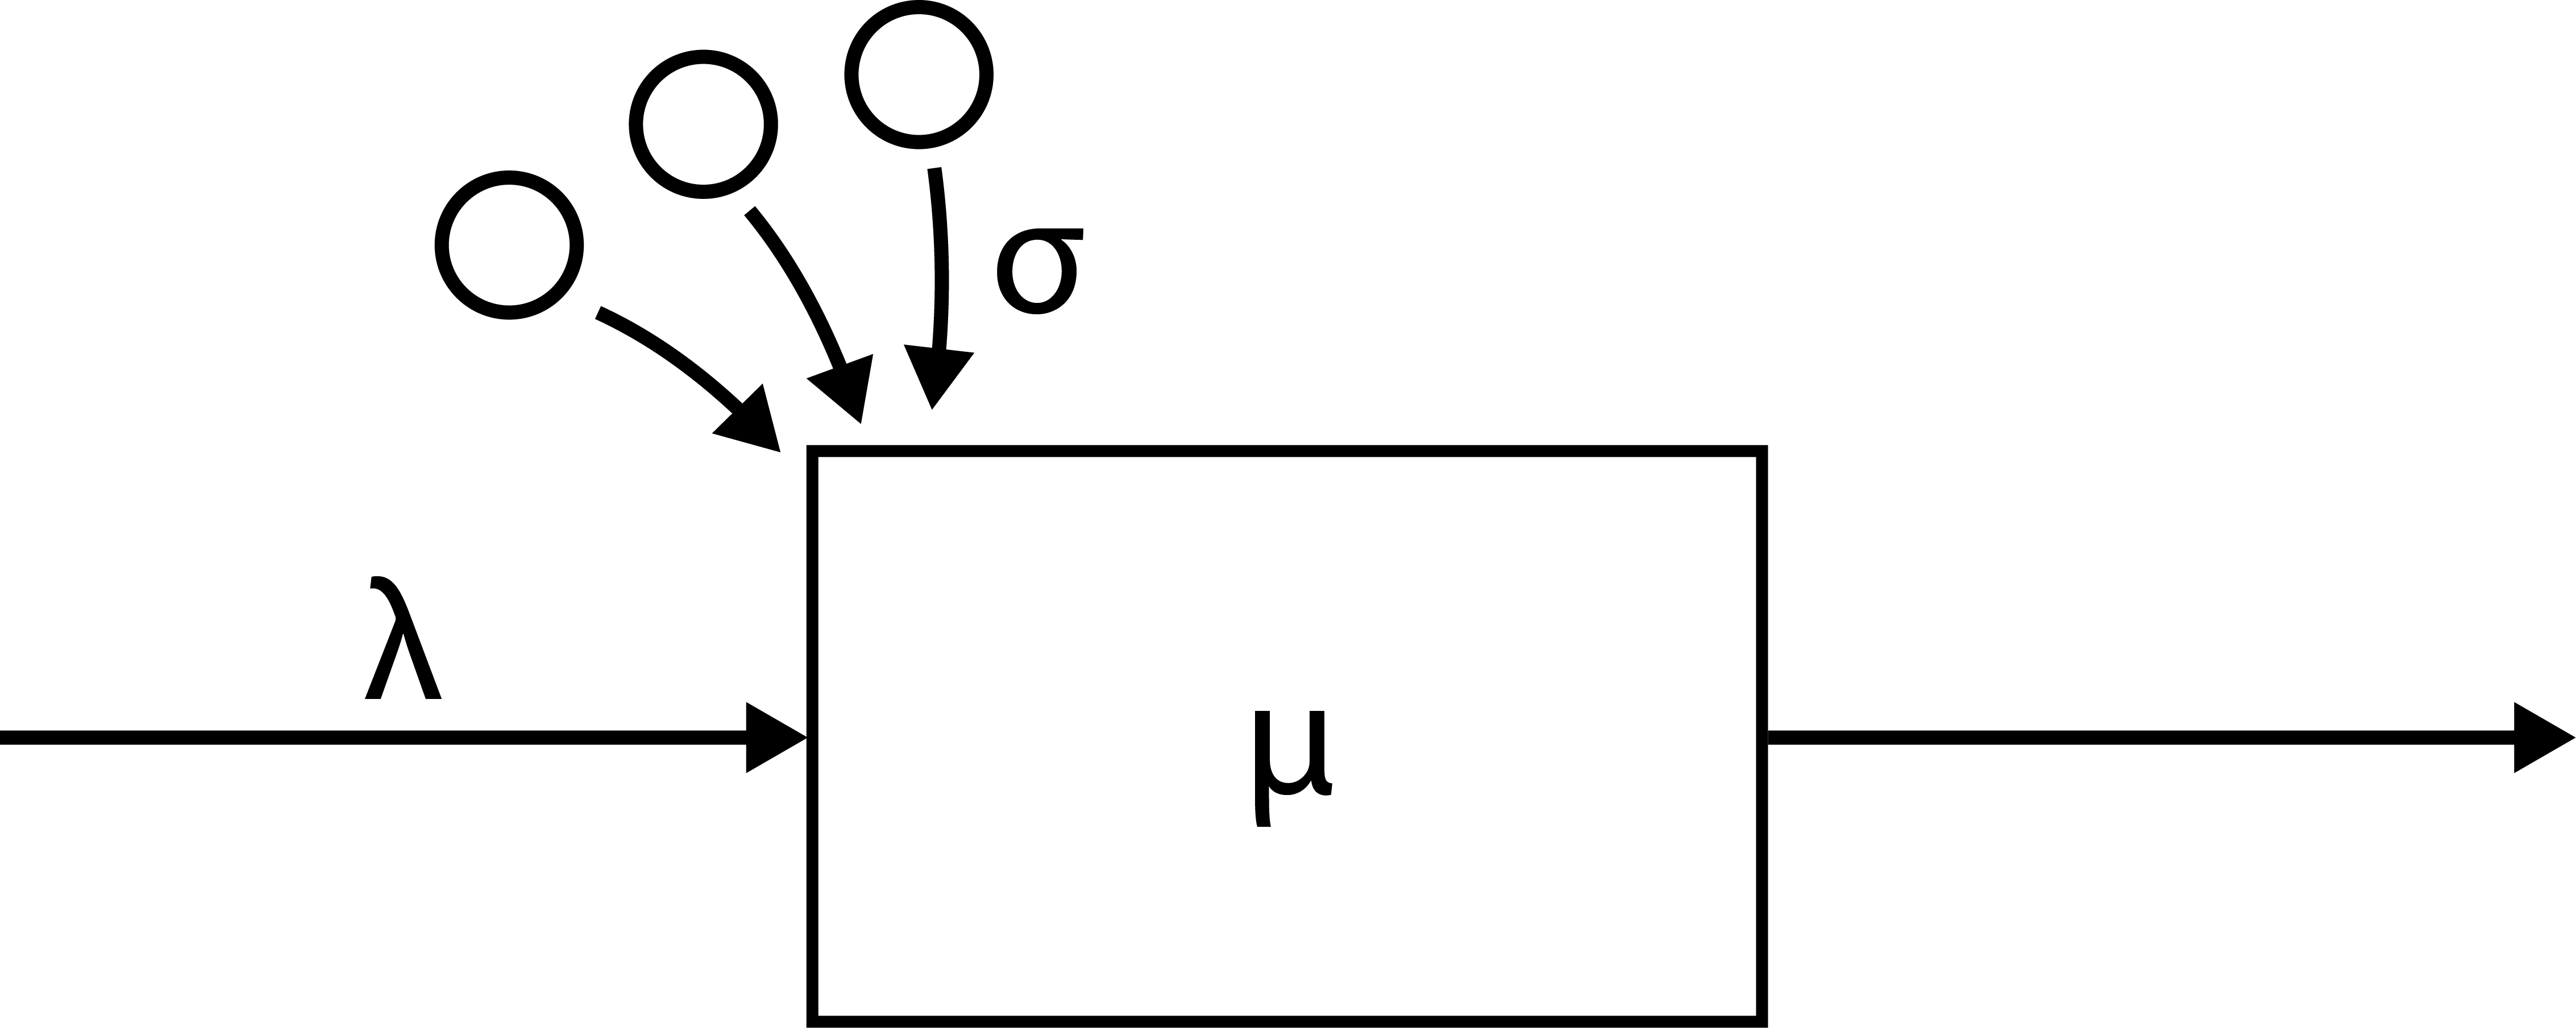
\includegraphics[scale=1,width=\textwidth]{1_sim_example.png}
	\caption{Пример системы ТМО}
	\label{sys_tmo_example}
\end{figure}

Алгоритм моделирования функционирования представленной системы массового обслуживания при помощи очереди событий представлен ниже.
Введем следующие обозначения:
\begin{enumerate}
	\item $Q$ --- очередь, хранящая моменты наступления предстоящих событий в системе и функционирующая по принципу кучи, когда извлекаемый элемент является минимальным среди содержащихся в ней;
	\item $T_{curr}$ --- текущее время моделирования;
	\item $T_{end}$ --- момент окончания моделирования;
	\item $t_i$ --- момент наступления события $i$ в системе. 
	\end{enumerate}

\begin{figure}[H]
	\centering
	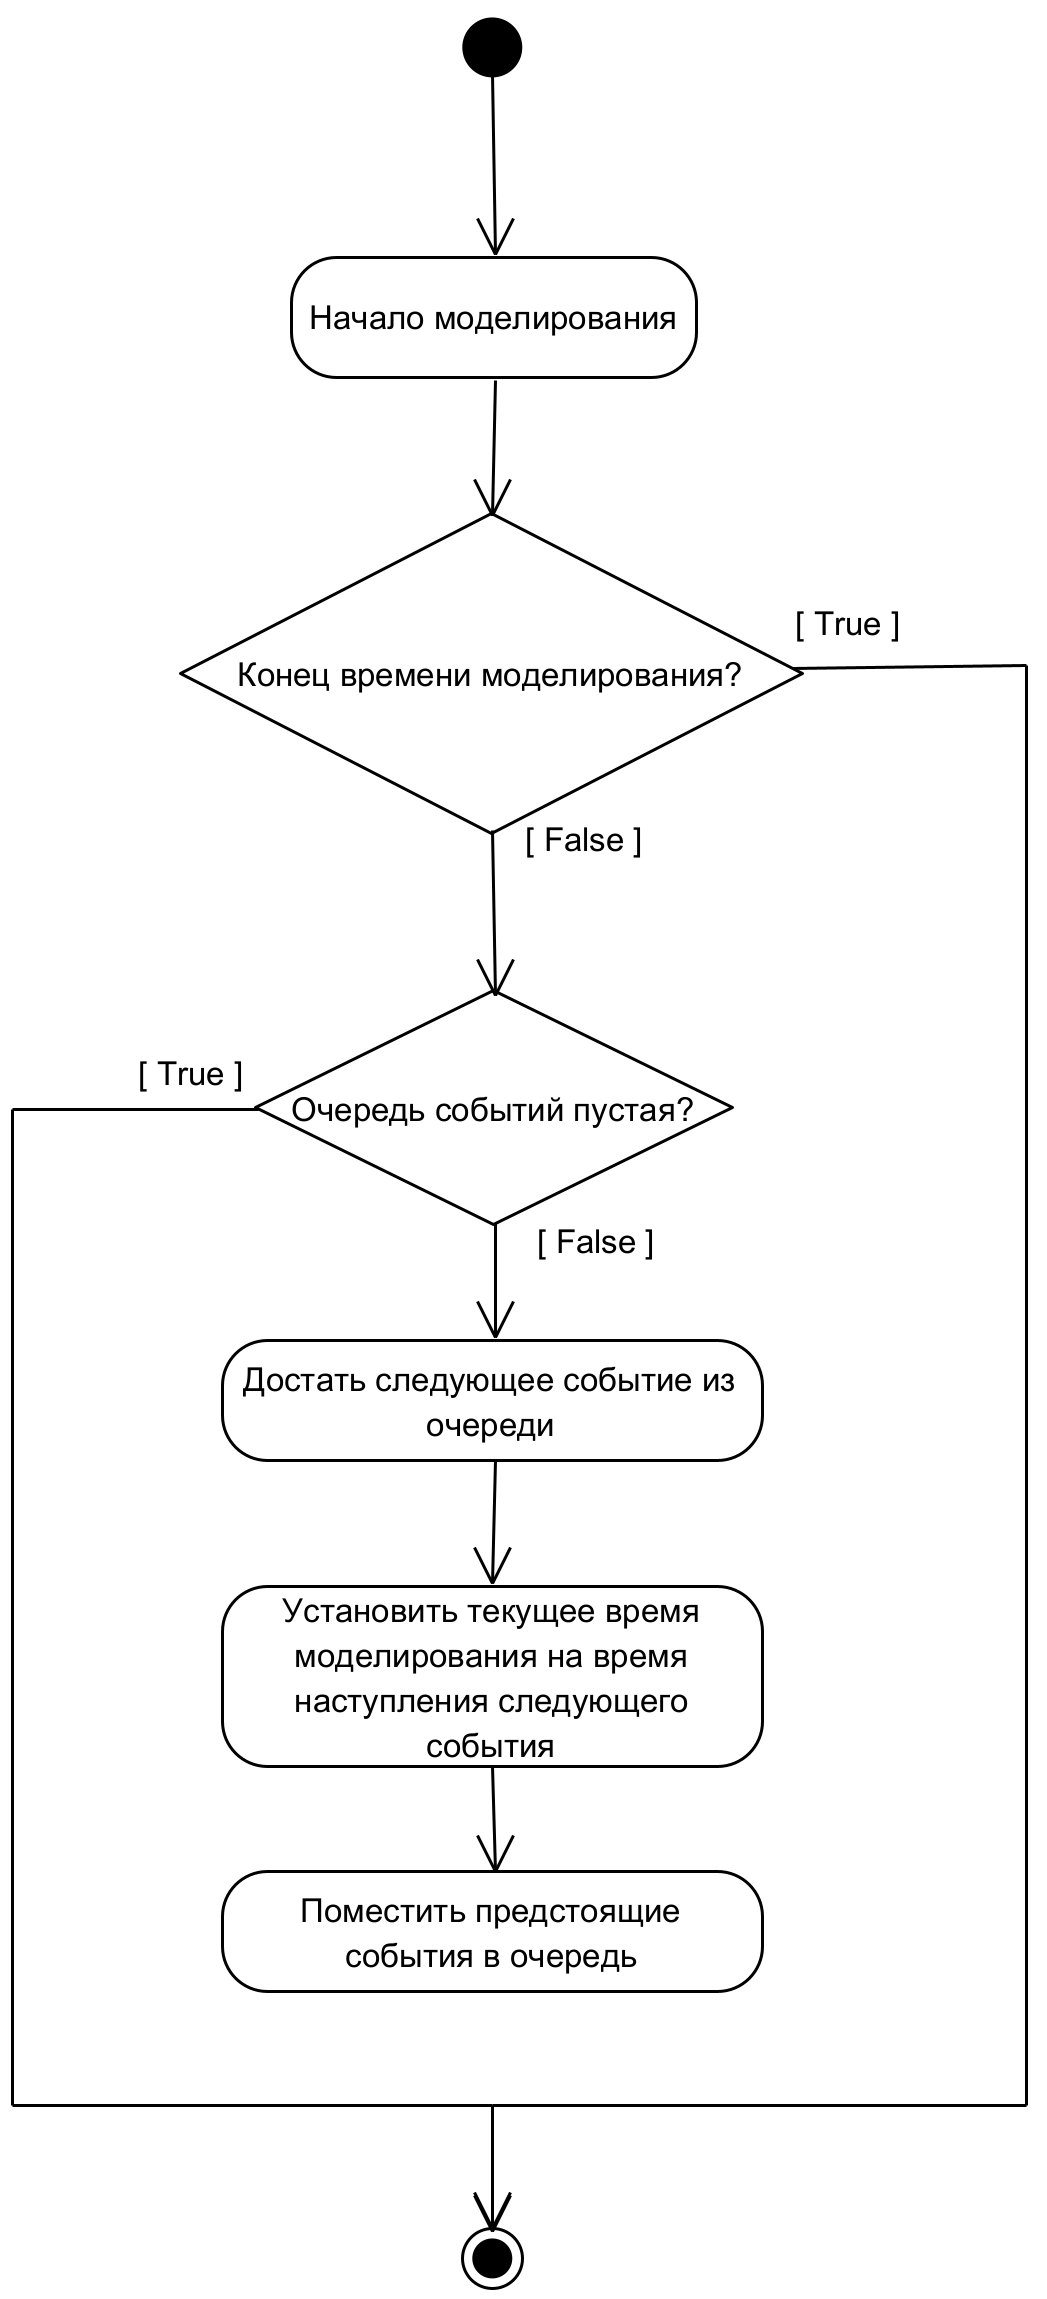
\includegraphics[scale=0.35]{sim_algo.png}
	\caption{Алгоритм моделирования}
	\label{sys_tmo_algo}
\end{figure}

Так, при каждой итерации моделирования из $Q$ достается момент наступления следующего события $t_i$, в свою очередь текущее время моделирования устанавливается как $T_{curr} = t_i$. Наступление события $i$ позволит получить время наступления последующего события $t_j$ (например, заявка успешно поступила на прибор из входящего потока в момент $t_i$, и $t_j$ будет являться момент окончания ее обслуживания), которое поместить в $Q$ и итерация алгоритма завершится, и процесс будет повторятся, пока $Q$ опустеет, либо $T_{curr} = T_{end}$.

Однако для получения достоверных результатов при помощи имитационного моделирования требуется достаточный объем выборки данных, получаемый при работе алгоритма \cite{лобач2004имитационное,моисеев2016исследование}. Определение требуемого объема выборки является отдельной подготовительной задачей и может решаться эмпирически путем подбора такого количества итераций алгоритма, при котором погрешность моделирования, выражаемая, к примеру, среднеквадратическим отклонением \cite{алиев2013погрешности}, становится несущественной.

Так как моделирование подразумевает сравнение получаемой выборки, в частности законов ее распределения, для проверки некой гипотезы о соответствии исследуемой математической модели, также требуется набор критериев и метрик для этого. В общем случае такой метрикой сравнения распределений может выступать расстояние Колмогорова, являющимся максимальной по модулю разницей между распределениями вероятностей:
\begin{equation}\label{kdistance}
	\Delta = \underset{0 < i < \infty}{max}\bigg\rvert \sum_{v=0}^{i} (P_0(v) - P_1(v))\bigg\rvert.
\end{equation}
Данная формула также применима для случаев с многомерными распределениями вероятностей \cite{fasano1987multidimensional}. Помимо распределений можно находить и сравнивать разные числовые характеристики системы: коэффициент загруженности системы, среднее время обслуживания, соотношение потерянных заявок и обслуженных, соотношение времени работы системы и числа успешно обслуженных заявок. Перечисленные характеристики нетрудно получить при моделировании. Это дает возможность делать косвенные выводы о других аспектах работы системы, которые еще не получены аналитически, но доступны к изучению на основе наблюдений при моделировании. В таком случае, численные методы могут выступать как более приоритетные при решении задач, когда исследуемые характеристики наблюдаемы, но аналитически невыводимы.
